


\chapter*{Introducción} 
\addcontentsline{toc}{chapter}{Introducción} 

Dentro de principales objetivos de de la sismología se encuentra el estudio
de los sismos y las causas que lo producen. Para cumplir este objetivo una de las
tareas más importantes en un observatorio sismológico es la localización de
fuentes sísmicas: Esto significa determinar tanto las coordenadas del hipocentro
como el tiempo de origen de dichos eventos sísmicos.

Asumiendo la respuesta sísmica del medio existen modelos matemáticos que nos
permiten estimar por medio de un conjunto de señales registradas ante la
ocurrencia de un micro sismo los parámetros del hipocentro y además, aunque de
forma inestable, cararterizar el sismo modelada como una fuerza modulada en el
tiempo. %% enviar este parrafo al aspecti físico del problema a resolver

El presente trabajo de título en si con un doble objetivo: Por un lado el diseño
algorítmico para la localización de hipocentros sísmico, tiempo de origen y
caracterización las fuentes sísmicas. Por otra parte es la automatización de
este proceso de estimación mediante un conjunto de implementaciones
computacionales que ofrece una interfaz para que cuyas funcionalidades puedan
ser empleadas en un software.

Estos modelos y alqgoritmos fueron aplicados en el contexto de la minería
subterránea a partir de las mediciones sísmicas disponibles. Los datos con que
se testeó el modelo y la implementación fueron obtenidos de las mediciones de
sismicidad de distintas minas de explotación subterránea de la división el
teniente, Codelco.

Se dividió este trabajo en los siguientes capítulos:
Capítulo I (Planteamiento del problema): La teoría sísmica y la interpretación
de las mediciones sismográficas suficiente para la comprensión de la
problemática.
Capítulo II (Marco teórico) Se analizó desde la teoría de la elasticidad cuyas
ecuaciones nos permite modelar los fenómenos sísmicos para un medio elástico,
homogéneo e infinito y permite deducir la función de Green la cual es esencial
para el diseño del algoritmo planteado en este trabajo.
Capítulo IIb: A partir de los datos de entrenamiento se diseña una red neuronal
que estima el tiempo de ocurrencia de la onda $P$ y la onda $S$.
Capítulo III: Se describe el modelos numérico para resolver el problema, basado
en los resultados expuestos en el capítulo II, este capítulo describe el modelo
y algoritmo matemático que permitirá la estimación del hipocentro sísmico usando
toda la información de la señal de los sismogramas, esto es una innovación con
respecto los actuales algoritmos que hacen una estimación del hipocentro
mediante el tiempo de arribo de la onda p y s, aunque usa esta estimación como
condición inicial. En esta parte de describirá el concepto de problema inverso y
una técnica para aplicarlo al problema elástico. Se justificara la demanda
computacional que involucra.
Capítulo IV: Se describirá el algoritmo y estructura de datos que se seleccionó
para resolver el problema y su versión computacional.
Capítulo V: está reservado para la descripción la versión computacional actual
de la solución, o sea, la implementación del método, la arquitectura de software
que se idónea que  según actuales autores se enmarca en el área de Big Data y
Ciencia de los Datos.
Capítulo VI: se describe la calidad del modelo y sus futuras aplicaciones,
posibles mejoras y recomendaciones.

Anexo A están los desarrollos matemáticos para los modelos físicos considerados
en este trabajo. En el Anexo B están las pruebas para sismos sintéticos.q

\begin{figure}
\centering
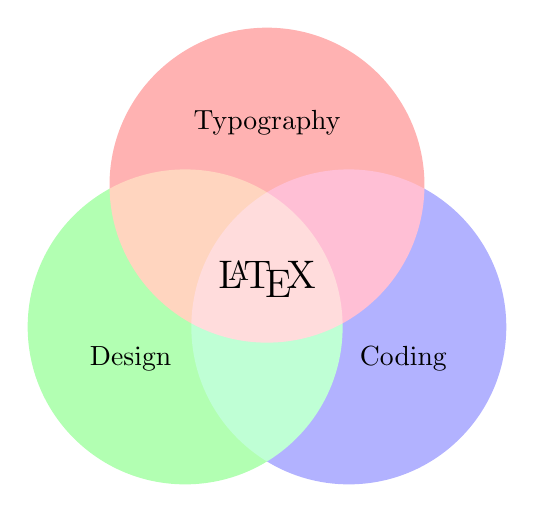
\begin{tikzpicture}
  \begin{scope}[blend group = soft light]
    \fill[red!30!white]   ( 90:1.2) circle (2);
    \fill[green!30!white] (210:1.2) circle (2);
    \fill[blue!30!white]  (330:1.2) circle (2);
  \end{scope}
  \node at ( 90:2)    {Typography};
  \node at ( 210:2)   {Design};
  \node at ( 330:2)   {Coding};
  \node [font=\Large] {\LaTeX};
\end{tikzpicture}
\end{figure}


\chapter{Justificación del tema} 

\section{Objetivos}

\subsection{General}

Formular un algoritmo basado en problemas inversos y redes neuronales para la
estimación de epicentros de los microsismos captados en las operaciones mineras
de El Teniente, Codelco. Basado en las mediciones sísmicas recojidas de los
sismogramas dispuestos en distintas locaciones de las zonas de extracción
subterranea.


\subsection{Específico}

\begin{enumerate}
  \item Desarrollar un método de conversión de datos a estructuras de datos
  \item Elaborar un método basado en redes neuronales para determinar el
  tiempo de llegada de la onda P y S de un sismo para una medición sismográfica.
  \item Estimar por medio de los resultados anteriores una ubicación del
  hipocentro para un evento sísmico.
  \item Reconstruir la fuerza puntual que caracteriza a un microsismo mediante
  un método numérico basado en modelos inversos.
  \item Modelar computacionalmente todos los puntos anteriormente expuestos en
  una librería de caracter científica.
\end{enumerate}


\subsection{Justificación del tema}
\subsubsection{Motivación}

\subsection{Alcances y limitaciones}

\subsection{Metodología y plan de trabajo}

\subsection{Resultados esperados}

